\documentclass[10pt]{standalone}
\usepackage{tikz}
\usetikzlibrary{arrows.meta}
\usepackage{unicode-math}
\setmainfont{XITS}
\setmathfont{XITS Math}
\begin{document}
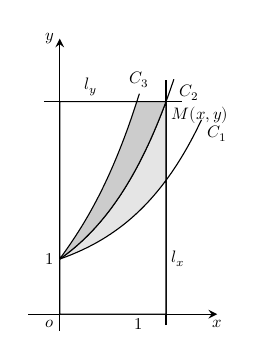
\begin{tikzpicture}[yscale=0.7]
\draw[-stealth] (-0.4,0)--(2,0) node[below,scale=0.6]{$x$};
\draw[-stealth] (0,-0.3)--(0,5) node[left,scale=0.6]{$y$};
\draw (0,0) node [below left,scale=0.6] {$o$};
\foreach \i in {1}{\draw (\i,0)--node [below,scale=0.6] {$1$}(\i,0.05);}
\draw (0,1) node [left,scale=0.6] {$1$};
\draw (1.35,1) node [right,scale=0.6] {$l_x$};
\draw (0.4,3.85742) node [above,scale=0.6] {$l_y$};
\draw (1.35,-0.2) -- (1.35,4.25519);
\draw (-0.2,3.85742) -- (1.55,3.85742);
\draw (1.35,3.85742) node [below right,scale=0.6] {$M(x,y)$};
%\clip (-1,-1) rectangle (5,5);%只在这个区域内画图
\draw[domain=1:4,smooth,variable=\t] plot ({ln(\t)+1/(2*\t)-0.5},\t)node[above,scale=0.6] {$C_3$};
\draw[domain=0:1.8,smooth] plot (\x,{0.5*1+0.5*exp(\x)}) node[below right,scale=0.6] {$C_1$};
\draw[domain=0:1.45,smooth] plot (\x,{exp(\x)}) node[below right,scale=0.6] {$C_2$};
\filldraw [fill=gray!20] (0,0) -- plot [domain=0:1.35,smooth] (\x,{exp(\x)}) -- (1.35,0) -- (0,0);
\filldraw [fill=white] (0,0) -- plot [domain=0:1.35,smooth] (\x,{0.5*1+0.5*exp(\x)}) -- (1.35,0) -- (0,0);
\filldraw [fill=gray!40] (0,1) -- plot [domain=0:1.35,smooth] (\x,{exp(\x)}) -- (0,3.85742) -- (0,1);
\filldraw [fill=white] (0,1) -- plot [domain=1:3.85742,smooth,variable=\t] ({ln(\t)+1/(2*\t)-0.5},\t) -- (0,3.85742) -- (0,1);
\end{tikzpicture}
\end{document}